\documentclass[a4paper,12pt]{report}
\usepackage[utf8]{inputenc} 
\usepackage{graphicx}
\graphicspath{ {Imagenes/} }
\usepackage{titlesec}
\setcounter{secnumdepth}{4}
\begin{document}

\tableofcontents

Mencionar:
Cambiar SNMP por OVS

\chapter{Pruebas}
\section{Motivación}
Uno de los principales objetivos del proyecto es realizar pruebas funcionales y de escala sobre la arquitectura del prototipo. Es de interés generar realidades distintas, y así detectar puntos de falla o variables clave en la performance de la arquitectura. Para esto se puede utilizar dos parámetros: topología y servicios. Es importante poder aplicar topologías complejas y relativamente grandes a la arquitectura, así como cantidades grandes de servicios para probar qué niveles de tráfico o flujos soporta el sistema antes de fallar o ver su performance reducida drásticamente. Dado que no es realista hacer este tipo de pruebas con un prototipo físico, por temas económicos y prácticos, se observó la necesidad de un entorno virtual capaz de simular las características del prototipo.

\chapter{Entorno virtual}
Uno de los principales objetivos de este trabajo es realizar pruebas funcionales y de escala sobre la arquitectura del prototipo. Es de interés generar distintas realidades, y así detectar puntos de falla o variables clave en la performance de la arquitectura. Para esto se puede utilizar dos parámetros: topología y servicios. Es importante poder aplicar topologias complejas y relativamente grandes a la arquitectura, así como grandes cantidades de servicios, y de esta forma encontrar posibles problemas con la arquitectura, y su respectiva solución. Dado que no es realista hacer este tipo de pruebas con un prototipo físico, por temas económicos y prácticos, se observa la necesidad de un entorno virtual capaz de simular las características del prototipo.

\section{Requerimientos del entorno virtual}
Los requerimientos de este entorno se pueden dividir en dos grupos. En primer lugar, la idea es que el entorno virtual se comporte de una forma lo más fiel posible al prototipo físico. Esto no quiere decir que deba usar las mismas herramientas, pero es deseable que así sea. En segundo lugar, hay que considerar los requerimientos inherentes de un entorno de simulación como el que se pretende. El primer grupo se detalla a continuación.

\begin{itemize}
	\item Se debe poder simular múltiples RAUSwitch virtuales, y los mismos deben tener las mismas capacidades funcionales que sus pares físicos. A partir de esto, se desprenden los siguientes sub-requerimientos.
	\begin{itemize}
		\item Deben poder ejecutar el protocolo de enrutamiento OSPF. Es deseable que lo hagan mediante la suite de ruteo Quagga.
		\item Deben soportar el protocolo OpenFlow 1.3. Esto se debe a que la aplicación que implementa VPNs depende de que los switches tengan soporte para MPLS, y OpenFlow ofrece esta funcionalidad a partir de la versión 1.3 (???). Es muy deseable que lo hagan mediante OpenVSwitch, ya que es lo que utilizan los RAUSwitch físicos.
	\end{itemize}
	\item Se debe poder simular múltiples hosts, ya que son los agentes que se conectan a la red y se envían tráfico entre sí, para corroborar que los flujos de datos son correctos.
	\item La aplicación RAUFlow debe ejecutarse y comunicarse correctamente con los RAUSwitch. Esto implica que el controlador Ryu debe ser soportado por el entorno.
\end{itemize}

Cabe remarcar que los módulos SNMP y LSDB Sync quedan por fuera de los requerimientos principales, por ser no esenciales. \\

El segundo grupo de requerimientos es más genérico, ya que son los que surgen para casi cualquier entorno de simulación de redes.

\begin{itemize} 
	\item Facilidad de configuración. Es importante que el entorno pueda generar distintas topologias y escenarios sin demasiado esfuerzo de configuración.
	\item Escalabilidad. Dado que uno de los objetivos es realizar pruebas de escala, el entorno debería ofrecer buena escalabilidad. Esto se traduce a que una computadora promedio de uso personal pueda levantar algunas decenas de nodos virtuales como mínimo.
\end{itemize}

\section{Elección de la herramienta}
Se estudió el estado del arte en lo que respecta a opciones de emulación o simulación para SDN. A continuación se detallan las principales herramientas analizadas al momento de hacer esta investigación.\\

\textbf{NS-3}\\
ns-3 fue descartado debido a que no ofrece soporte para Quagga ni OpenFlow 1.3 al momento de realizar esta investigacion.\\

\textbf{Estinet}\\
Estinet requiere licencias pagas, y se opto por elegir herramientas open source. Debido a la falta de documentación de libre acceso, no se sabe que tipo de capacidades ofrece.\\

\textbf{Mininet}\\
Mininet es un emulador de redes SDN que permite emular hosts, switches, controladores y enlaces. Utiliza virtualización basada en procesos para ejecutar múltiples instancias (hasta 4096) de hosts y switches en un unico kernel de sistema operativo. También utiliza una capacidad de Linux denominada \textit{network namespace} que permite crear "interfaces de red virtuales", y de esta manera dotar a los nodos con sus propias interfaces, tablas de ruteo y tablas ARP. Lo que en realidad hace Mininet es utilizar la arquitectura \textit{Linux container}, que tiene la capacidad de proveer virtualización completa, pero de un modo reducido ya que no requiere de todas sus capacidades. Mininet también utiliza \textit{virtual ethernet (veth)} para crear los enlaces virtuales entre los nodos.


\textbf{LXC}\\
La opción de crear nodos con Linux containers resuelve el problema de Quagga y OpenFlow 1.3, pero llevaría una gran cantidad de trabajo construir distintas topologias (sobre todo si son grandes), ya que casi todo debe ser configurado manualmente por el usuario. Es una opción similar a Mininet, solo que sin gozar de todas las facilidades que ofrece esta última.\\


\textbf{Máquinas virtuales}\\
Es una opción similar a LXC (Linux Containers), sólo que menos escalable.
\\

\section{Diseño e implementación del entorno}
El entorno está construido alrededor de Mininet, y se podría pensar como una extensión de la misma. \textit{Out of the box}, Mininet ya cumple tres de los cuatro requerimientos explicados anteriormente. Está diseñada para ser escalable, ya que usa containers reducidos, tiene soporte para OpenFlow 1.3 mediante OpenVSwitch, y es muy fácil de usar. El aspecto en el que falla es en el soporte para Quagga. Dado que Mininet es una herramienta de prototipado para SDN puro, no está pensado para un esquema híbrido como el que se propone. Los switches compatibles con OpenVSwitch que ofrece no pueden tener su propio network namespace, por lo tanto, no pueden tener su propia tabla de ruteo ni interfaces de red aisladas, así que no es posible que utilicen Quagga.

Por otro lado, los hosts de Mininet sí tienen su propio network namespace, y gracias a su capacidad de tener sus propios procesos y directorios, podemos ejecutar una instancia de Quagga y OpenVSwitch para cada host. De esta forma es posible crear un router como el requerido por la arquitectura. Esta extensión de las funcionalidades de los hosts es posible ya que Mininet está programado con orientación a objetos y permite al usuario crear subclases propias de las clases que vienen por defecto. En la figura \ref{fig:clases_entorno} se puede ver la estructura de clases del entorno construido. En las siguientes secciones se procederá a estudiar cada una de ellas.

\begin{figure}[t]
	\caption{Diagrama de clases del entorno.}
	\includegraphics[scale=0.65]{Entorno/clases_entorno}
	\centering
	\label{fig:clases_entorno}
\end{figure}

\subsection{RAUController}
En el uso típico de Mininet, la comunicación entre el controlador y el switch se da a través de la interfaz de loopback. Esto es así porque los switches no tienen su propio namespace. Para lograr dicha comunicación, no hace falta un objeto en Mininet que represente el controlador, ya que ejecutar la aplicación en el sistema operativo base ya habilita al switch a comunicarse con ella a través de la interfaz de loopback. Esta situación cambia en este diseño, porque los switches pasan a tener su propio network namespace. Esto lleva a la necesidad de crear un host virtual, que ejecute la aplicación de RAUFlow y se comunique con los switches a través de enlaces virtuales. Para satisfacer esta necesidad se usa la clase RAUController.

\subsection{RAUSwitch}
La clase RAUSwitch es el núcleo del entorno de simulación. Es un Host extendido de tal forma para que, gracias a la funcionalidad de directorios privados, ejecute su propia instancia de Quagga y OpenVSwitch. Cada RAUSwitch tiene los siguientes directorios privados: /var/log/, /var/log/quagga, /var/run, /var/run/quagga, /var/run/openvswitch. Cada RAUSwitch también usa un directorio bajo /tmp, para almacenar sus archivos de configuración.\\ \\

OpenVSwitch básicamente consiste de 2 demonios (ovs-vswitchd y ovsdb-server) que ejecutan en el user-space, y un módulo en el kernel que actúa como cache para los flujos recientes. Utiliza el protocolo 'netlink' para comunicar el user-space con el módulo en el kernel. Poder tomar decisiones sobre los paquetes a nivel del kernel, sin tener que pasar por el user-space, explica en gran medida el buen nivel de performance que ofrece OpenVSwitch. Sin embargo, tener múltiples módulos de kernel ejecutando en el mismo sistema operativo puede crear comportamientos impredecibles e incorrectos, ya que no está previsto para trabajar de esa forma.\\
Afortunadamente, OpenVSwitch puede ejecutarse completamente en modo user-space, es decir, sin soporte del módulo del kernel. Esto implica que podemos ejecutar tantas instancias de OpenVSwitch como queramos, pero la performance va a ser significativamente peor. Esto no es una desventaja muy seria, ya que el objetivo del entorno no es ser performante al procesar paquetes. Cabe aclarar que en este modo OpenVSwitch continúa haciendo cacheo de flujos, pero ahora lo hace en el user-space.

\begin{figure}[t]
	\caption{Arquitectura de OpenVSwitch.}
	\includegraphics[scale=0.65]{Entorno/ovs_dataplane}
	\centering
	\label{fig:ovs_dataplane}
\end{figure}

\subsection{QuaggaRouter}
Es una clase similar al RAUSwitch pero sin OpenVSwitch, es decir, sólo usa Quagga. Apunta a representar el router CE que utilizaría una subred para conectarse a la red. Está conectado a un RAUSwitch de borde.

\subsection{RAUHost}
Es una clase auxiliar, sin ninguna particularidad. Sirve para evitar determinadas configuraciones manuales, como por ejemplo, el \textit{default gateway}.



\chapter{Pruebas de escala}
Con el entorno de simulación construido, el siguiente objetivo es realizar pruebas de escala sobre la arquitectura. Este trabajo consiste de dos etapas. La primera sección explica la primera de ellas, que es verificar que la arquitectura funciona para topologias de escala. Habiendo completado esta etapa, se pasa a realizar estudios de escala sobre la cantidad de servicios. En este capítulo se explicará el propósito de cada prueba, las condiciones bajo las cuales se ejecuta cada una de ellas (topologias, tipos de tráfico, etc) y por último, los resultados que arrojan. Todas las pruebas fueron realizadas en una máquina virtual con 3590 MB de RAM, procesador Intel Core i5-5200u y Lubuntu 14.04 como sistema operativo.

\section{Topologias de escala}
Es importante poder asegurar que la arquitectura puede ser fácilmente migrada a redes reales. Para poder asegurar esto, es necesario comprobar que topologias con grandes cantidades de nodos no generan problemas inesperados. Dado que en el proyecto RRAP se contaba con cuatro dispositivos, este tipo de pruebas no han sido realizadas hasta el momento.

\subsection{Descripción del escenario}
Este escenario consiste de una VPN punto a punto de capa 3. Dicha VPN permite tráfico de ethertype \textbf{0x0800}, es decir, tráfico del protocolo IPv4. Se utilizarán distintas topologias, pero la estructura de la prueba será similar siempre:
\begin{itemize}
	\item Dos subredes cliente. Serán implementadas por un QuaggaRouter y un RAUHost cada una (recordar las clases del entorno virtual). Los RAUHost serán los remitentes y destinatarios del tráfico que pasará por la VPN. Esos datos se generarán con el comando \textit{ping} y la herramienta \textit{iperf}.
	\item El controlador, implementado por el RAUController. Éste se conectará con un switch genérico (gracias a la clase Switch de Mininet, en el modo \textit{standalone}), que a su vez se conectará con los RAUSwitch. Esta será la red de gestión. Por simplicidad, dicha red se omitirá en las futuras imágenes.
	\item La red de RAUSwitch, conectados de acuerdo a lo que dicte cada topología.
\end{itemize}
Los aspectos que se buscan verificar con esta prueba son los siguientes: \\ \\
\textbf{Algoritmo de ruteo} \\
 Se verifican dos aspectos claves: que el camino se corresponde con el camino esperado (calculado previamente de forma manual), y que el camino es correctamente instalado en forma de reglas de reenvío (en base a conmutación de etiquetas MPLS) en las respectivas tablas de flujos OpenFlow de cada nodo del camino. Todo esto se puede comprobar analizando las tablas de flujos de cada nodo, que se pueden ver utilizando el comando \textbf{dump-flows} de OpenVSwitch. También se puede utilizar la interfaz gráfica de RAUFlow. Desde las tablas de flujos se puede reconstruir el camino que computó la aplicación, y también comprobar que los flujos configuran correctamente las etiquetas MPLS. \\ \\
\textbf{Clasificación de tráfico} \\
La idea es verificar que realmente se están asignando las etiquetas MPLS al tráfico entrante, así como comprobar que el mismo es reenviado por los nodos correctos. Se genera tráfico utilizando el comando \textbf{ping} y la herramienta \textbf{iperf}. Con la herramienta tcpdump, se verifica el tráfico que pasa por cada nodo del camino. \\ \\
Las topologias que se usarán son:
\begin{itemize}
	\item \textbf{Básica}: 4 nodos en topología de full mesh. Es la utilizada en el prototipo físico.
	\item \textbf{Chica}: topología arbitraria de 11 nodos (fuente: Topology Zoo). Figura \ref{fig:topo_chica}.
	\item \textbf{Mediana}: topología arbitraria de 45 nodos (fuente: Topology Zoo). Figura \ref{fig:topo_mediana}.
	\item \textbf{Grande}: topología de tipo arborescente compuesta por 100 nodos.
\end{itemize}

\begin{figure}[t]
\caption{Topología chica}
\includegraphics[scale=0.4]{Pruebas/topo_chica}
\centering
\label{fig:topo_chica}
\end{figure}

\begin{figure}[t]
\caption{Topología mediana}
\includegraphics[scale=0.15]{Pruebas/topo_mediana}
\centering
\label{fig:topo_mediana}
\end{figure}

\subsection{Resultados y observaciones}
En general, se observa que la aplicación no tiene problemas para manejar grandes cantidades de nodos, pero sí caminos largos. A continuación se desglosa el resultado de la prueba con cada topología. El mismo también se puede ver en la tabla \ref{table:problemas_por_topologia}. En ella se indica con una X los aspectos que funcionaron correctamente para cada caso. Los aspectos que se estudian son: se crea con éxito el servicio desde la interfaz web, el camino que se instala es correcto, los flujos de cada nodo del camino son correctos, y se clasifica correctamente el tráfico. Si se cumplen todos ellos, se puede concluir que la topología pasa la prueba.

\begin{table}[ht]
\caption{Resultados por topología.}
% title of Table
\centering 
% used for centering table
\begin{tabular}{c c c c c}
\hline\hline
Largo del camino & Servicio & Camino & Flujos  & Clasificación de tráfico \\ [0.5ex]
\hline
1 & X & X & X & X \\
7 & X & X &  &  \\
10 &  &  &  &  \\
X &  &  &  &  \\ [1ex]
\hline
\end{tabular}
\label{table:problemas_por_topologia}
\end{table}

\begin{itemize}
	\item \textbf{VPN con camino de 1 salto, en la topología básica}. La VPN se establece correctamente y el tráfico ICMP y TCP pasa sin problemas.
	\item \textbf{VPN con camino de 7 saltos, en la topología chica}. Los servicios se crean, y se instalan flujos en los nodos correctos, osea que el camino calculado es el más corto. Sin embargo, los flujos instalados en los nodos son incorrectos.
	\item \textbf{VPN con camino de 10 saltos, en la topología mediana}. La aplicación sufre una excepción de Python al crear los servicios.
	\item \textbf{VPN con camino de X saltos, en la topología grande}. La aplicación sufre una excepción de Python al crear los servicios, igual que el caso anterior (???).
\end{itemize}
\textbf{Bug en codigo (ruta)} \\
EXPLICAR: Error en el código que hacía que se instalaran mal los flujos en los nodos. Tenian incorrectos puertos de entrada y salida.\\
\textbf{Bug en codigo (Dijkstra)} \\
EXPLICAR: Error en el código del algoritmo de Dijkstra que hacia que se calcularan mal los costos, ya que se sumaba como strings (concatenación) en vez de sumar enteros. \\
\textbf{Problema del MTU al usar iperf} \\
EXPLICAR: Hay que reducir 5 o 10 bytes (dependiendo de si el servicio usa 1 o 2 niveles de etiquetas MPLS) al MTU para que el tráfico pase.\\




Probar ancho de banda y tiempo de creación de servicios para cada topología y cada largo de camino. Así quedan dos tablas.

\section{Escala de servicios y flujos}
Entre los requerimientos de la RAU2 se encuentra el de la escalabilidad de usuarios. En particular, se espera alcanzar en un mediano plazo un total de 11.000 docentes, 7.000 funcionarios y 140.000 estudiantes. Esto implica que la red será sujeta a importantes cantidades de servicios y flujos distintos. He aquí la relevancia de las pruebas en la presente sección. Mediante el entorno virtual, se someterá la arquitectura a una cantidad de servicios relativamente grande y de esta forma se podrán identificar posibles puntos de falla, o umbrales bajo los cuales debe mantenerse la red para funcionar con buen rendimiento. Dado que en esta prueba también se utilizarán topologias grandes, hay que recordar la misma es posible gracias a la corrección de los errores que se explicó en la sección anterior. También es importante recordar que aunque el entorno de simulación permite hacer un valioso estudio de escalabilidad, no generará resultados en lo que refiere a la performance de la arquitectura. Recordar sección 3.3.2, donde se explica que cada instancia de Open vSwitch se ejecuta en modo user-space, y por ende procesa los paquetes de forma bastante lenta.

\subsection{Descripción del escenario}
Este escenario es muy similar al anterior. Se utiliza una VPN punto a punto de capa 3 para conectar dos subredes cliente, y se utiliza \textit{iperf} para generar tráfico TCP y medir el ancho de banda entre los dos RAUHost. Para cargar a la arquitectura con servicios, se crean múltiples VPN de capa 2 entre las subredes, variando los cabezales OpenFlow para que toda VPN sea distinta de las demás. De esta forma, existirán múltiples VPN pero solo una (la de capa 3) será utilizada. \\
Dado que cargar todas las VPN a mano en la interfaz web llevaría demasiado tiempo, se creó un servicio web que recibe como parámetro la cantidad de VPN que se desean y se encarga de crearlas. \\ \\
\begin{figure}[t]
	\caption{Topología para prueba de escala de servicios.}
	\includegraphics[scale=0.15]{Pruebas/stress_servicios_topologia}
	\centering
	\label{fig:stress_servicios_topologia}
\end{figure}
El objetivo es verificar los siguientes dos aspectos claves: \\ \\
\textbf{Escalabilidad interna del RAUSwitch} \\
Se estudian posibles limitaciones internas que puedan tener los dispositivos, cuando deben manejar grandes cantidades de flujos. Es posible que a medida que crece su tabla de flujos, demoren más en encontrar el flujo que se corresponde con cada paquete que reciben. Si pasa esto, el ancho de banda debería ser afectado negativamente por la cantidad de flujos en sus tablas. El ancho de banda se medirá con la herramienta \textit{iperf}.  \\ \\
\textbf{Escalabilidad en servicios} \\
Se estudian posibles problemas que puedan tener la arquitectura de la red o la aplicación del controlador para manejar grandes cantidades de servicios e información. \\ \\
Esta prueba se repite para las mismas topologias que la prueba anterior, es decir: básica (4 nodos), chica (11 nodos), mediana (45 nodos) y grande (100 nodos).

\subsection{Resultados y observaciones}

\begin{table}[ht]
	\caption{Anchos de banda, en Kbits/s, medidos para cada caso.}
	\centering 
	\begin{tabular}{c c c c c}
		\hline\hline
		\# de VPN & Básica & Chica & Mediana  & Grande \\ [0.5ex]
		\hline
		1 & X & Y & W & Z \\
		3000 & X & Y & W & Z  \\
		6000 & X & Y & W & Z \\
		9000 & X & Y & W & Z \\
		12000 & X & Y & W & Z \\
		15000 & X & Y & W & Z \\ [1ex]
		\hline
	\end{tabular}
	\label{table:escala_de_servicios}
\end{table}

Los resultados de la prueba con cada topología se puede ver en la tabla \ref{table:escala_de_servicios}. Se pueden observar dos hechos interesantes. El primer resultado que se puede estudiar, es que el ancho de banda es más bajo a medida que se incrementa la cantidad de nodos y/o el largo del camino. Esto se explica desde dos ángulos. El primero es que al tener que pasar por un camino más largo, el paquete debe ser inspeccionado y reenviado más veces. Por lo tanto, este resultado debería sería visible también en un ambiente de prueba con dispositivos físicos. El segundo ángulo que explica este resultado radica en el entorno virtual mismo. Al tener que manejar más nodos virtuales, el sistema operativo anfitrión tiene menos recursos para dedicar a cada uno. Esto quiere decir que tanto las instancias de \textit{iperf} que se encargan de recibir y enviar los paquetes, como las instancias de Open vSwitch que los procesan en cada nodo del camino, tendrán menos tiempo de CPU para realizar su tarea. \\

El otro resultado que se puede observar en la tabla \ref{table:escala_de_servicios}, es que el ancho de banda es constante para una topología, sin importar la cantidad de VPN existentes en el momento. Como se explica en el primer objetivo de esta prueba, se busca determinar si la existencia de muchos flujos en la tabla, implica que el switch OpenFlow demora más tiempo en encontrar el flujo que corresponde con un paquete entrante, y por lo tanto el mismo demora más en ser forwardeado. Si esto fuera así, debería haber un impacto directo en el throughput. El máximo de VPN con el que se probó fueron 15.000. Cada VPN de capa 2 está compuesta por dos servicios de capa 2, y cada uno de esos servicios introduce 42 flujos en cada nodo del camino. Esto quiere decir que cada uno contiene alrededor de 1.260.000 flujos en su tabla. \\
La explicación de porqué esa cantidad de flujos no afecta el ancho de banda se encuentra en la especificación de la herramienta Open vSwitch, que utiliza la arquitectura y el entorno virtual para implementar OpenFlow. Dicha herramienta realiza cacheo de flujos. Eso quiere decir que cuando un paquete de datos de un determinado flujo llega por primera vez a un nodo, este paquete es enviado al pipeline de OpenFlow para determinar qué acción se debe tomar. Luego de realizada, esta acción es escrita en la caché, y tiene un tiempo de vida de entre 5 y 10 segundos. Si en ese período de tiempo llega otro paquete del mismo flujo, no hay necesidad de enviar el paquete al pipeline, porque ya se sabe cuales son las acciones a tomar para ese paquete. Por lo tanto, si un flujo de datos es constante y rápido, el tamaño de la tabla de OpenFlow no afectará el tiempo de decisión, ya que sólo el primer paquete de ese flujo deberá pasar por el pipeline. \\
Mediante el comando 'ovs-appctl dpctl/show' de Open vSwitch, podemos examinar las estadísticas de la cache del datapath. Con el parámetro opcional \textit{target} se apunta el comando a cada instancia de Open vSwitch, y por ende, a cada nodo. En las figuras \ref{fig:iperf_sample} y \ref{fig:cache_sample} se observa, por un lado, la salida de 'iperf' luego de hacer tres ejecuciones, y por otro, las estadísticas del nodo 'alice' luego de dichas ejecuciones. En la sección 'lookups' se detallan cuantos 'hits' y 'miss' de caché han ocurrido hasta el momento, y 'flows' indica cuantos flujos activos hay en el momento en la caché. \\ \\
Otro objetivo de la prueba es determinar si la arquitectura, y en particular la aplicación, tienen algún problema para manejar muchos servicios. No se detectó ninguna problema de esa índole. Sin ser una limitación, pero sí un factor importante, hay que recordar que los datos que maneja el controlador (entre ellos, los servicios) están en memoria. Por lo tanto se podrá agregar servicios mientras la computadora subyacente tenga suficiente memoria. La creación de 15.000 VPN (30.000 servicios) aumenta el consumo de memoria del controlador en 412 Mb (CONFIRMAR), por lo que un servicio ocupa alrededor de 14 Kb. A modo de ejemplo, si extrapolamos ese número a una computadora que puede dedicar 4 Gb de RAM al controlador, llegamos a que dicho controlador podrá mantener alrededor de 300.000 servicios.


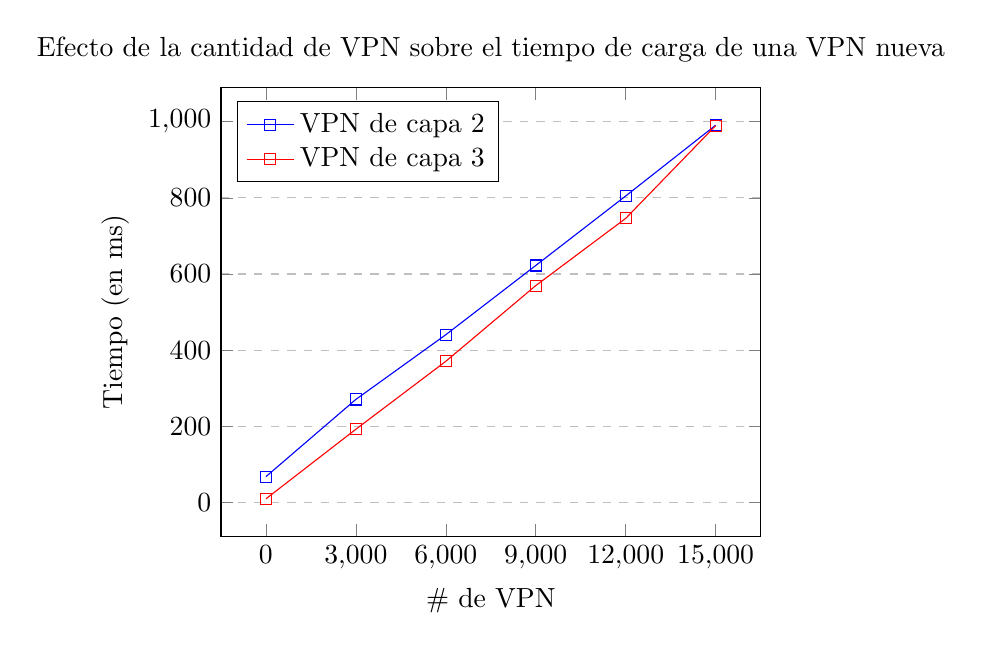
\begin{tikzpicture}
\begin{axis}[
	title={Efecto de la cantidad de VPN sobre el tiempo de carga de una VPN nueva},
	xlabel={\# de VPN},
	ylabel={Tiempo (en ms)},
	xtick={0,3000,6000,9000,12000,15000},
	ytick={0,200,400,600,800,1000,1200},
	scaled x ticks = false,
	x tick label style={/pgf/number format/fixed},
	legend pos=north west,
	ymajorgrids=true,
	grid style=dashed,
]
\addplot[
	color=blue,
	mark=square,
	]
	coordinates {
		(1,68.2)(3000,270.9)(6000,440.7)(9000,622.4)(12000,804.8)(15000,990.5)
	};
	\addlegendentry{VPN de capa 2}
\addplot[
	color=red,
	mark=square,
	]
	coordinates {
		(1,10.0)(3000,192.6)(6000,370.9)(9000,569.6)(12000,746.0)(15000,989.3)
	};
	\addlegendentry{VPN de capa 3}
\end{axis}
\end{tikzpicture}



Tiempo de carga de las VPNs aumenta a medida que hay mas VPNs?
Tiempo de carga de las VPNs aumenta a medida que hay mas nodos?

NUEVOS:

================================
Topo Basica
-
Memoria sin servicios: 0.9%
Uso de la CPU sin VPN: 3.0%
Ancho de banda sin VPN: 886 903 889 (receptor) 937 956 941 (emisor)
Tiempo de carga de una VPN de capa 3, sin VPN: 0.002513 segundos (ida) 0.007488 (vuelta)
Tiempo de carga de una VPN de capa 2, sin VPN: 0.033592 segundos (ida) 0.034675 (vuelta)
-
Memoria con 15.000 VPN: 11.5%
Uso de la CPU con 15.000 VPN: 67.8%
Tiempo para crear 15.000 VPN: 8238 segundos
Ancho de banda con 15.000 VPN: 884 886 887 (receptor) 936 939 938 (emisor)
Tiempo de carga de una VPN de capa 3, con 15.000 VPN: 0.499023 segundos (ida) 0.490338 (vuelta)
Tiempo de carga de una VPN de capa 2, con 15.000 VPN: 0.484804 segundos (ida) 0.505755 (vuelta)
-
Memoria con 3.000 VPN: 3.0%
Uso de la CPU con 3.000 VPN: 25.0%
Tiempo para crear 0-3.000 VPN: 500 segundos
Ancho de banda con 3.000 VPN: 899 882 880 (receptor) 900 932 931 (emisor)
Tiempo de carga de una VPN de capa 3, con 3.000 VPN: 0.096597 segundos (ida) 0.096071 (vuelta)
Tiempo de carga de una VPN de capa 2, con 3.000 VPN: 0.124546 segundos (ida) 0.146423 (vuelta)
-
Memoria con 6.000 VPN: 5.2%
Uso de la CPU con 6.000 VPN: 38.0%
Tiempo para crear 3.000-6.000 VPN: 1086 segundos
Ancho de banda con 6.000 VPN: 882 897 881 (receptor) 934 949 931 (emisor)
Tiempo de carga de una VPN de capa 3, con 6.000 VPN: 0.182752 segundos (ida) 0.188211 (vuelta)
Tiempo de carga de una VPN de capa 2, con 6.000 VPN: 0.220683 segundos (ida) 0.220042 (vuelta)
-
Memoria con 9.000 VPN: 7.2%
Uso de la CPU con 9.000 VPN: 47.5%
Tiempo para crear 6.000-9.000 VPN: 1629 segundos
Ancho de banda con 9.000 VPN: 896 882 893 (receptor) 898 934 895 (emisor)
Tiempo de carga de una VPN de capa 3, con 9.000 VPN: 0.279042 segundos (ida) 0.290570 (vuelta)
Tiempo de carga de una VPN de capa 2, con 9.000 VPN: 0.306835 segundos (ida) 0.315573 (vuelta)
-
Memoria con 12.000 VPN: 9.4%
Uso de la CPU con 12.000 VPN: 55.9%
Tiempo para crear 9.000-12.000 VPN: 2180 segundos
Ancho de banda con 12.000 VPN: 880 878 896 (receptor) 932 930 949 (emisor)
Tiempo de carga de una VPN de capa 3, con 12.000 VPN: 0.362166 segundos (ida) 0.383873 (vuelta)
Tiempo de carga de una VPN de capa 2, con 12.000 VPN: 0.412899 segundos (ida) 0.391985 (vuelta)


\begin{figure}[t]
	\caption{Estadísticas de cache de flujos del nodo 'alice'.}
	\includegraphics[scale=1]{Pruebas/cache_sample}
	\centering
	\label{fig:cache_sample}
\end{figure}

\begin{figure}[t]
	\caption{Resultado de la ejecución de 3 pruebas iperf en el host h1.}
	\includegraphics[scale=1]{Pruebas/iperf_sample}
	\centering
	\label{fig:iperf_sample}
\end{figure}



\end{document}